\chapter{Ride Management and Real-Time Interaction}

\section{Introduction}

Following the implementation of user authentication and profile management in Chapter 3, this chapter focuses on the core operational functionality of the platform: ride management and real-time interaction.

The objective is to enable users to create, search, and manage rides efficiently, while ensuring dynamic synchronization between participants through real-time communication mechanisms.

This chapter is structured according to the Scrum methodology and is divided into two main development phases:

\begin{itemize}
    \item \textbf{Sprint 3: Ride Management System} — implementation of ride creation, booking, and lifecycle management.
    \item \textbf{Sprint 4: Real-Time Interaction} — implementation of real-time communication using WebSocket technology.
\end{itemize}

Each sprint includes its product backlog, system design through UML diagrams, implementation details, user interface integration, and validation.

% =========================================================
\section{Sprint 3: Ride Management System}

\subsection{Sprint Objective}

The objective of this sprint is to implement the complete ride management workflow, allowing users to offer rides, search for available rides, book seats, and manage ride execution through a structured lifecycle.

\subsection{Product Backlog}

\begin{table}[H]
\centering
\begin{tabular}{|l|l|l|}
\hline
\textbf{User Story} & \textbf{Description} & \textbf{Priority} \\
\hline
US1 & Create a ride & High \\
US2 & Search for available rides & High \\
US3 & Book a ride & High \\
US4 & Cancel a booking & Medium \\
US5 & View ride details & High \\
US6 & Manage ride lifecycle & High \\
\hline
\end{tabular}
\caption{Sprint 3 Product Backlog}
\end{table}

\subsection{Use Case Diagram}

The main actor in this sprint is the \textbf{Collaborator}, who interacts with the ride system to perform ride-related operations.

\begin{figure}[H]
\centering
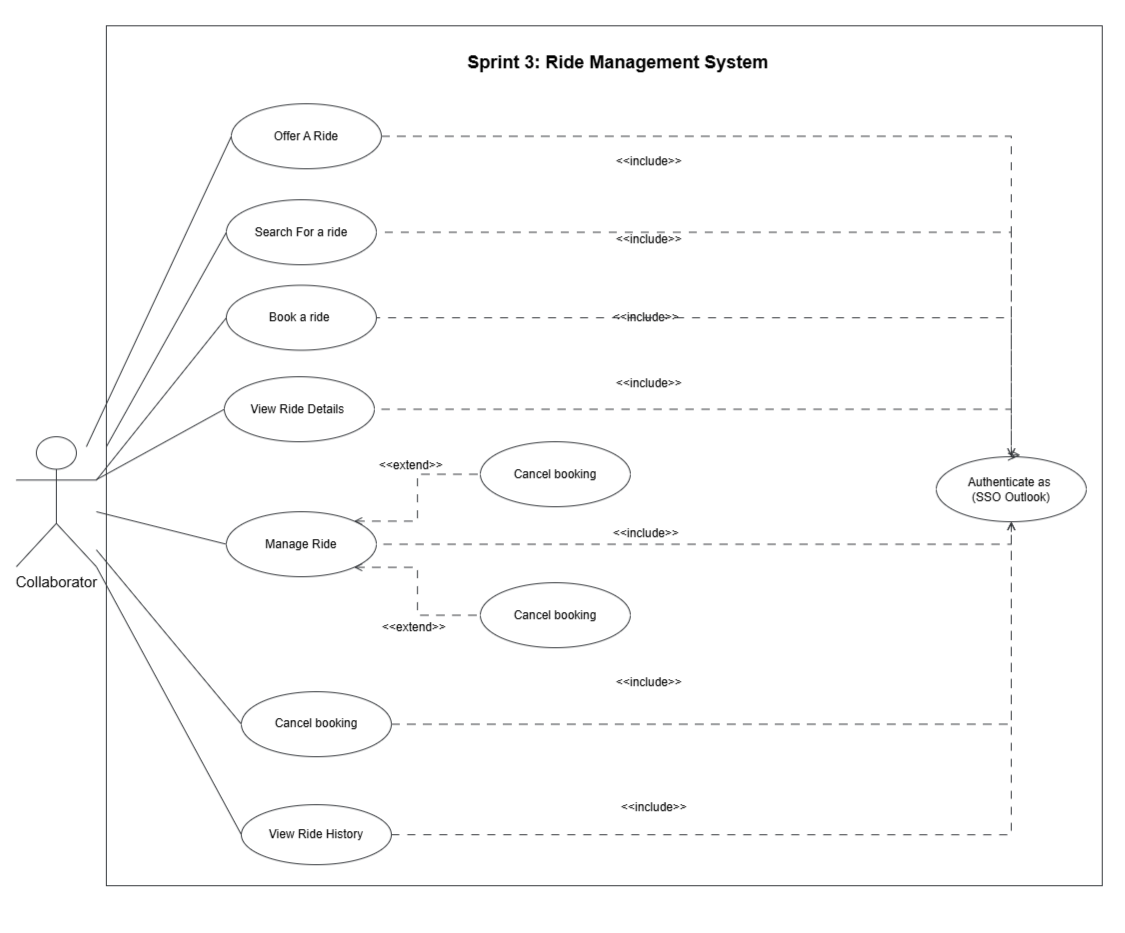
\includegraphics[width=0.8\textwidth]{images/diagrams/usecase_sprint3.png}
\caption{Use Case Diagram — Ride Management}
\end{figure}

\subsection{Sequence Diagram — Ride Booking}

The booking process ensures that constraints such as seat availability and ride validity are verified before confirming a reservation.

\begin{figure}[H]
\centering
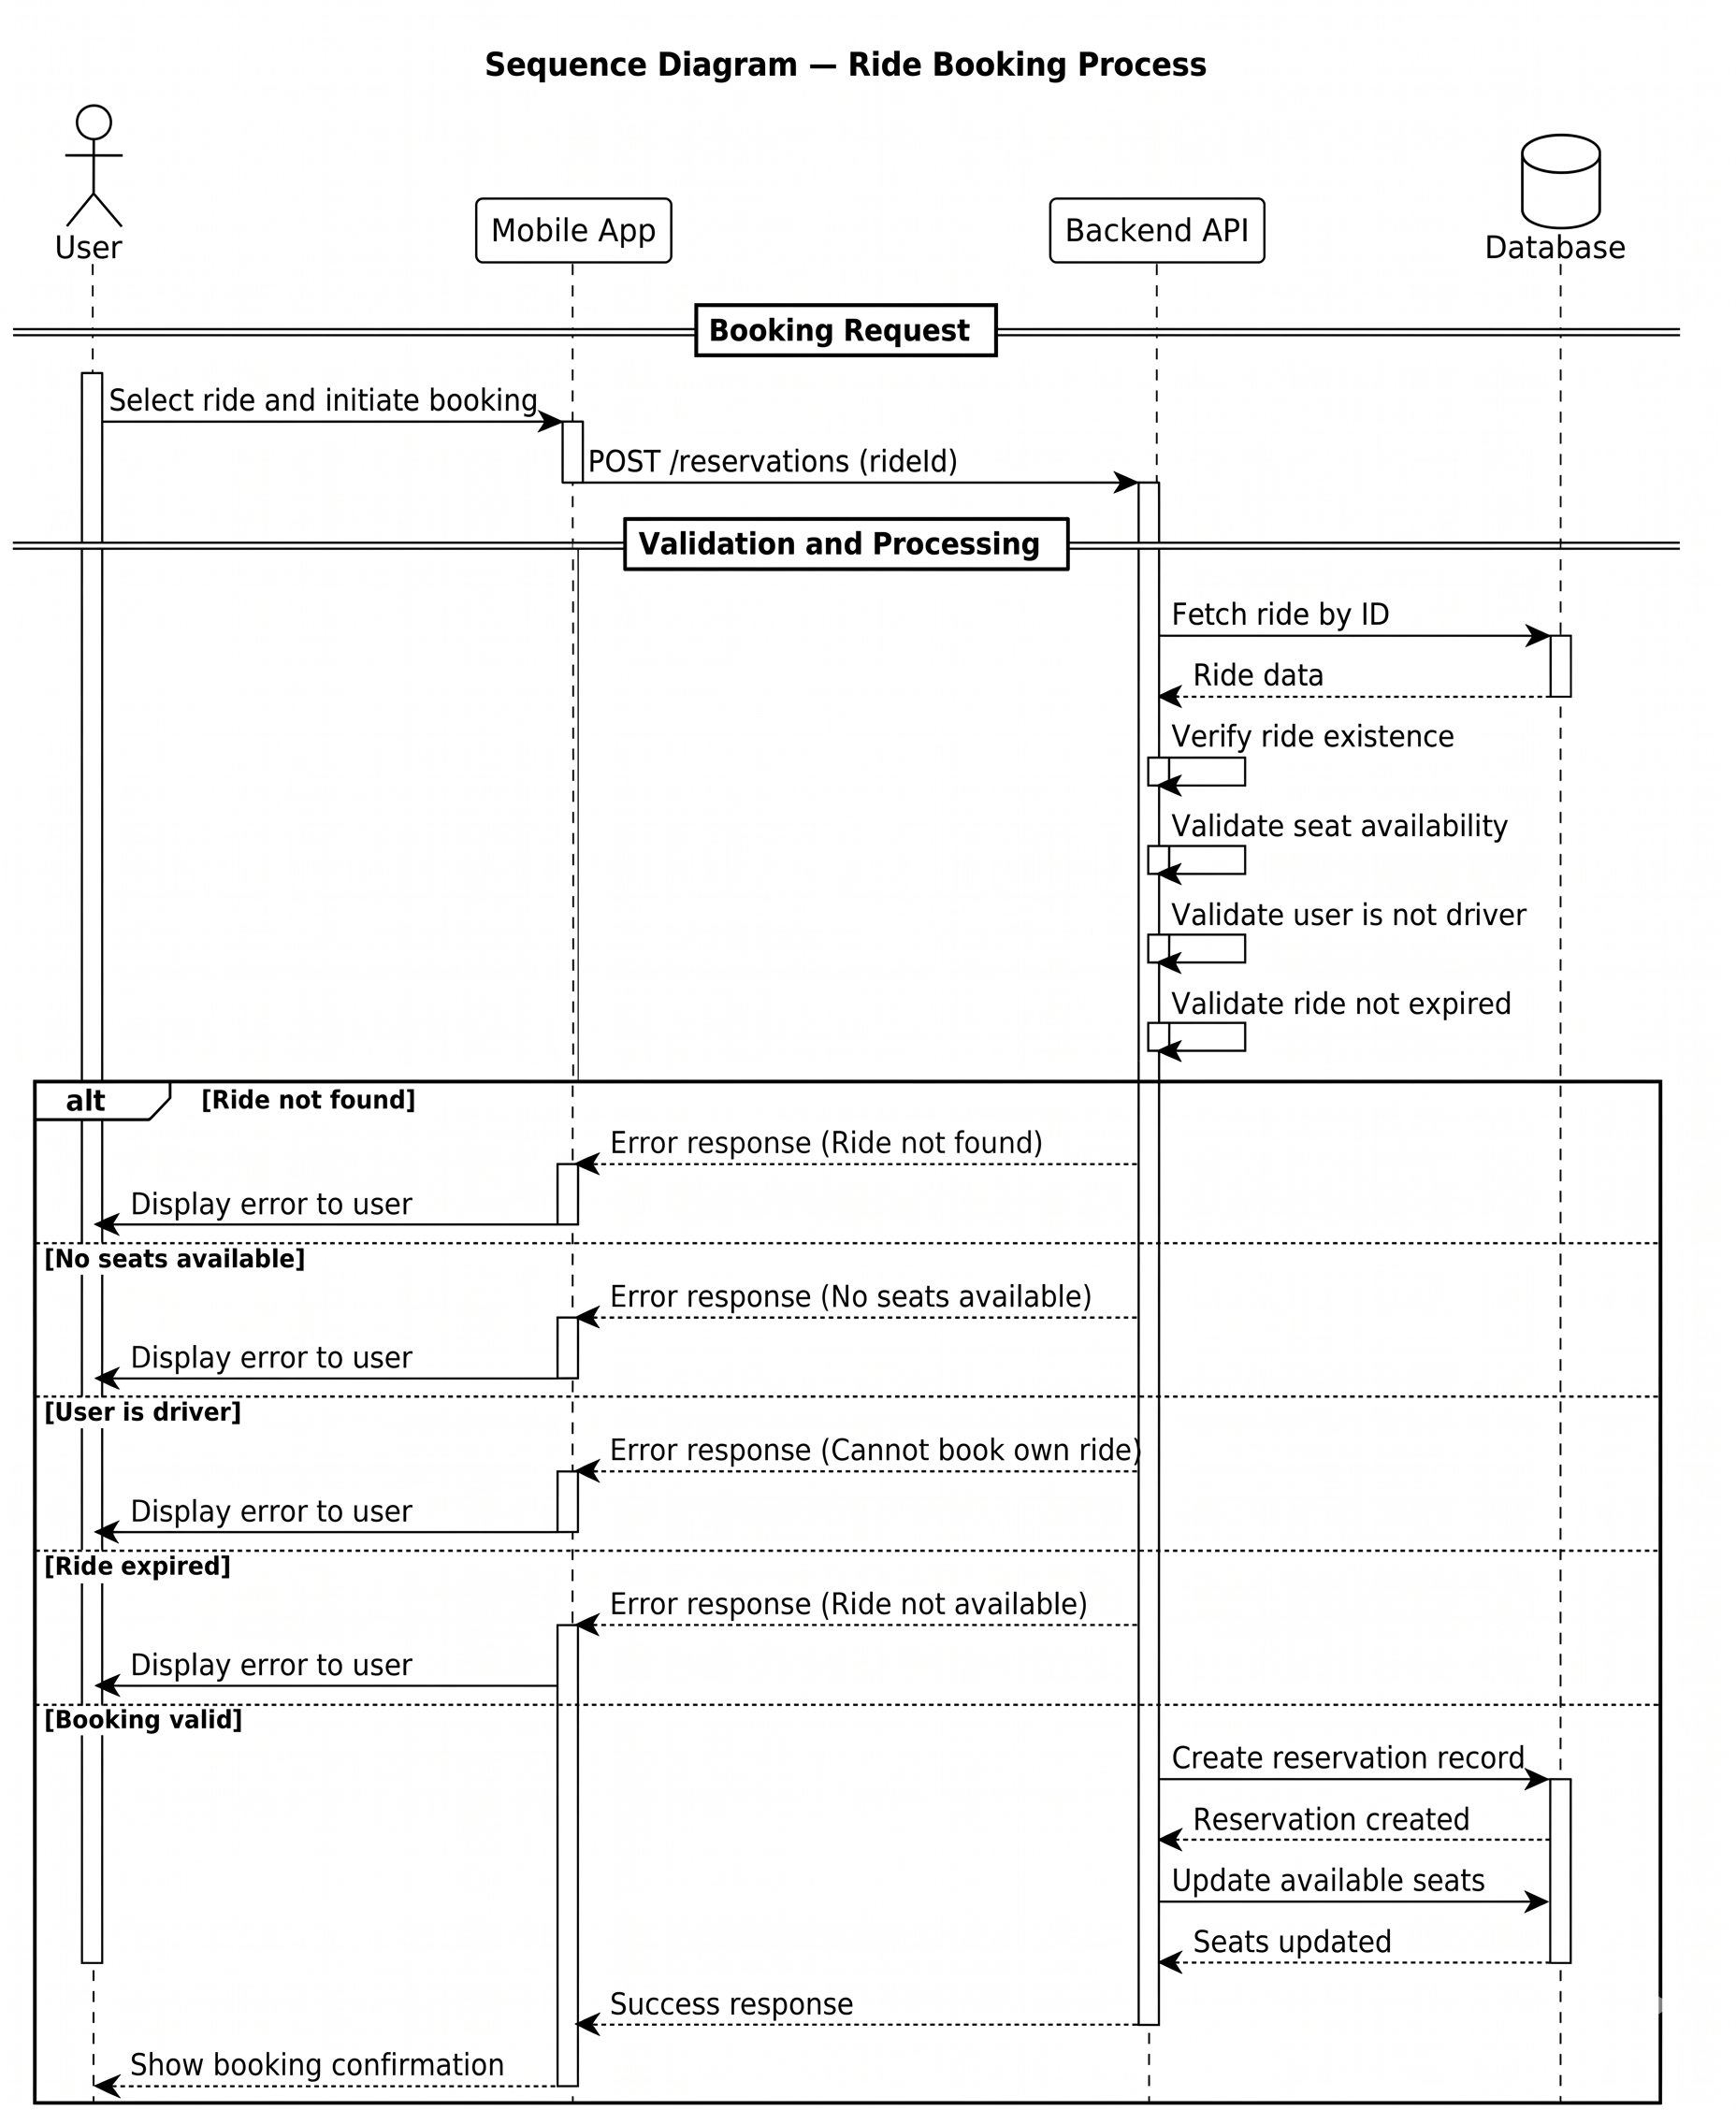
\includegraphics[width=0.9\textwidth]{images/diagrams/sequence_booking.png}
\caption{Sequence Diagram — Ride Booking Process}
\end{figure}

\subsection{Class Diagram}

The ride management system is based on three main entities: \textbf{User}, \textbf{Ride}, and \textbf{Reservation}.

\begin{figure}[H]
\centering
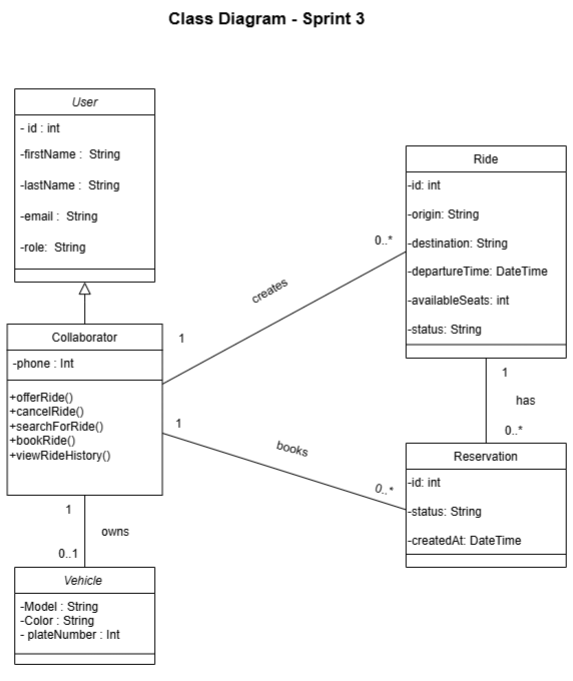
\includegraphics[width=0.85\textwidth]{images/diagrams/class_sprint3.png}
\caption{Class Diagram — Ride Management}
\end{figure}

\subsection{Ride Lifecycle Management}

The ride lifecycle is modeled as a finite state machine that defines the different stages of a ride from creation to completion.

The system supports the following states:

\begin{itemize}
    \item Scheduled
    \item Driver En Route
    \item Arrived
    \item In Progress
    \item Completed
    \item Cancelled
    \item Missed
\end{itemize}

Transitions between these states are triggered either by user actions (e.g., driver starting the ride) or automatically by the system (e.g., ride expiration).

\begin{figure}[H]
\centering
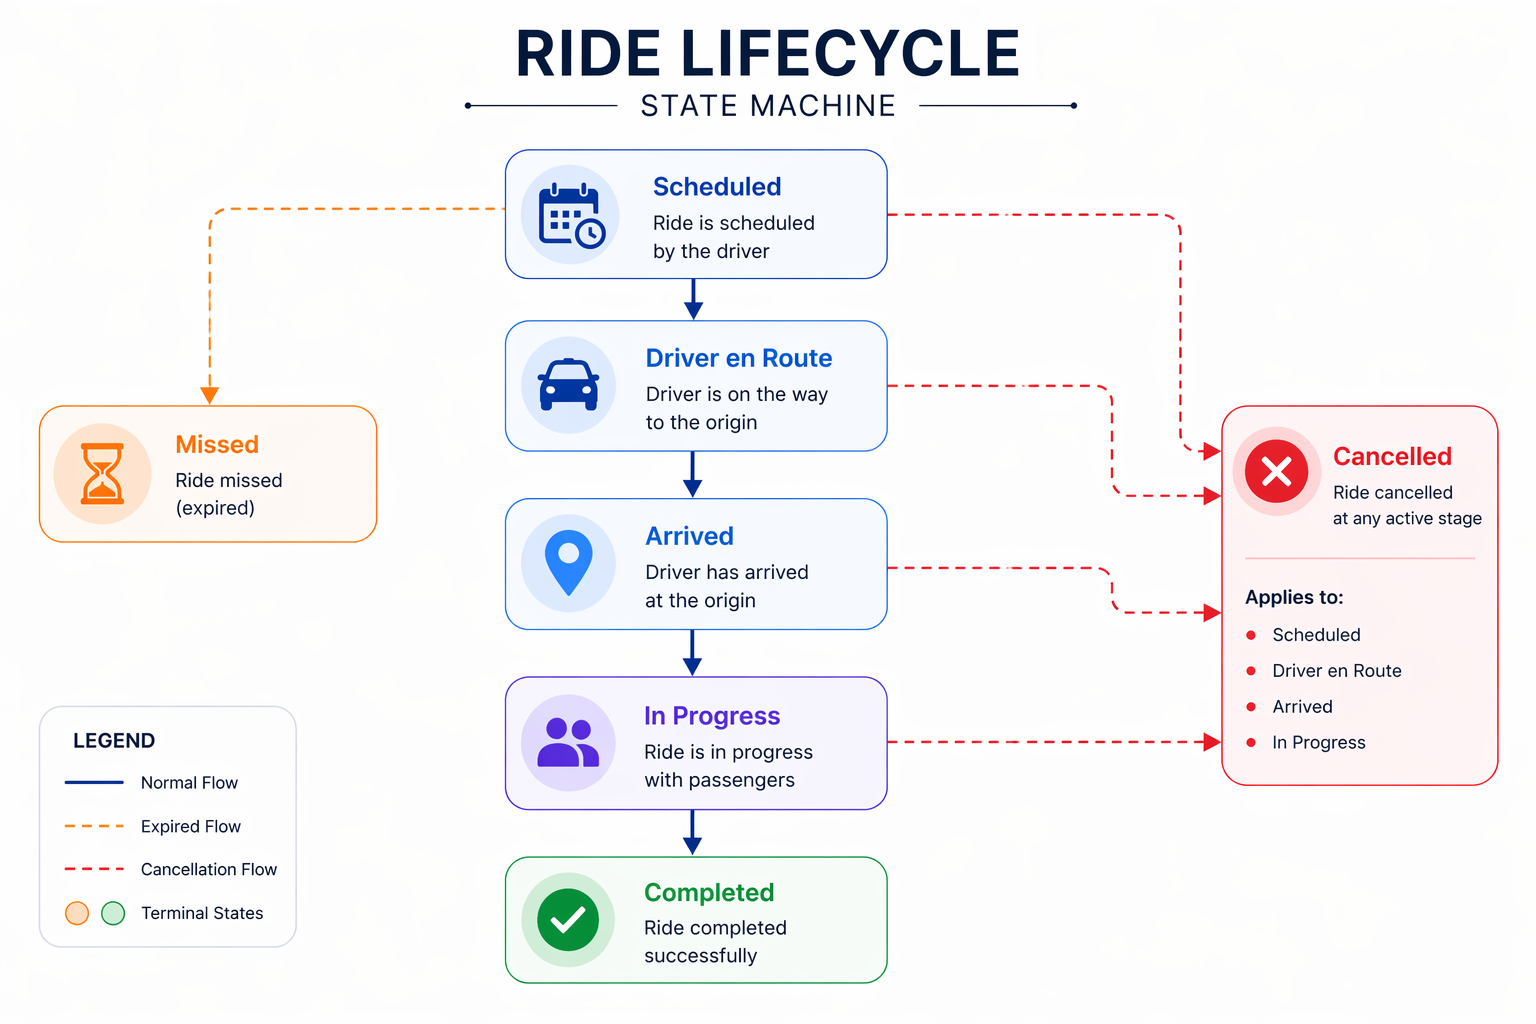
\includegraphics[width=0.85\textwidth]{images/architecture/ride_lifecycle.png}
\caption{Ride Lifecycle State Machine}
\end{figure}

This lifecycle ensures consistency in ride execution and enables the system to handle edge cases such as inactivity or missed departures.

\subsection{Business Rules}

To ensure system integrity, several business rules are enforced:

\begin{itemize}
    \item A user cannot book their own ride.
    \item The number of booked seats cannot exceed available capacity.
    \item A ride cannot be booked after its departure time.
    \item Reservations must be confirmed before the boarding deadline.
    \item A ride automatically transitions to \textit{missed} if the driver does not start it within the allowed time.
\end{itemize}

These constraints are validated at the backend level to guarantee consistency and reliability.

\subsection{User Interface Integration}

The implemented features are reflected in several user interface screens:

\begin{itemize}
    \item Ride creation screen
    \item Ride search screen
    \item Ride details screen
\end{itemize}

% \begin{figure}[H]
% \centering
% 
\includegraphics[width=0.4\textwidth]{images/chapter4/create_ride.png}
% \caption{Create Ride Interface}
% \end{figure}

% \begin{figure}[H]
% \centering
% 
\includegraphics[width=0.4\textwidth]{images/chapter4/search_ride.png}
% \caption{Search Ride Interface}
% \end{figure}

\subsection{Sprint Validation}

The system was validated using the following scenarios:

\begin{itemize}
    \item Successful ride creation
    \item Successful ride booking
    \item Booking rejection when no seats are available
    \item Ride cancellation and state update
\end{itemize}

Testing was performed at the end of the sprint to ensure functional correctness and system reliability.

% =========================================================
\section{Sprint 4: Real-Time Interaction}

\subsection{Sprint Objective}

The objective of this sprint is to enable real-time communication between users and the system, ensuring that ride status and driver location updates are instantly propagated.

\subsection{Product Backlog}

\begin{table}[H]
\centering
\begin{tabular}{|l|l|l|}
\hline
\textbf{User Story} & \textbf{Description} & \textbf{Priority} \\
\hline
US1 & Live ride status updates & High \\
US2 & Driver location tracking & High \\
US3 & Real-time synchronization & High \\
\hline
\end{tabular}
\caption{Sprint 4 Product Backlog}
\end{table}

\subsection{Real-Time Architecture}

The system uses WebSocket technology to establish persistent communication between the client and the server.

Unlike traditional HTTP communication, WebSocket enables bidirectional data exchange, allowing the server to push updates to clients instantly.

This architecture ensures low-latency updates and improves user experience during active rides.

\subsection{Sequence Diagram — Real-Time Update}

The real-time update mechanism follows an event-driven architecture where updates are emitted by the backend and received by connected clients.

\begin{figure}[H]
\centering
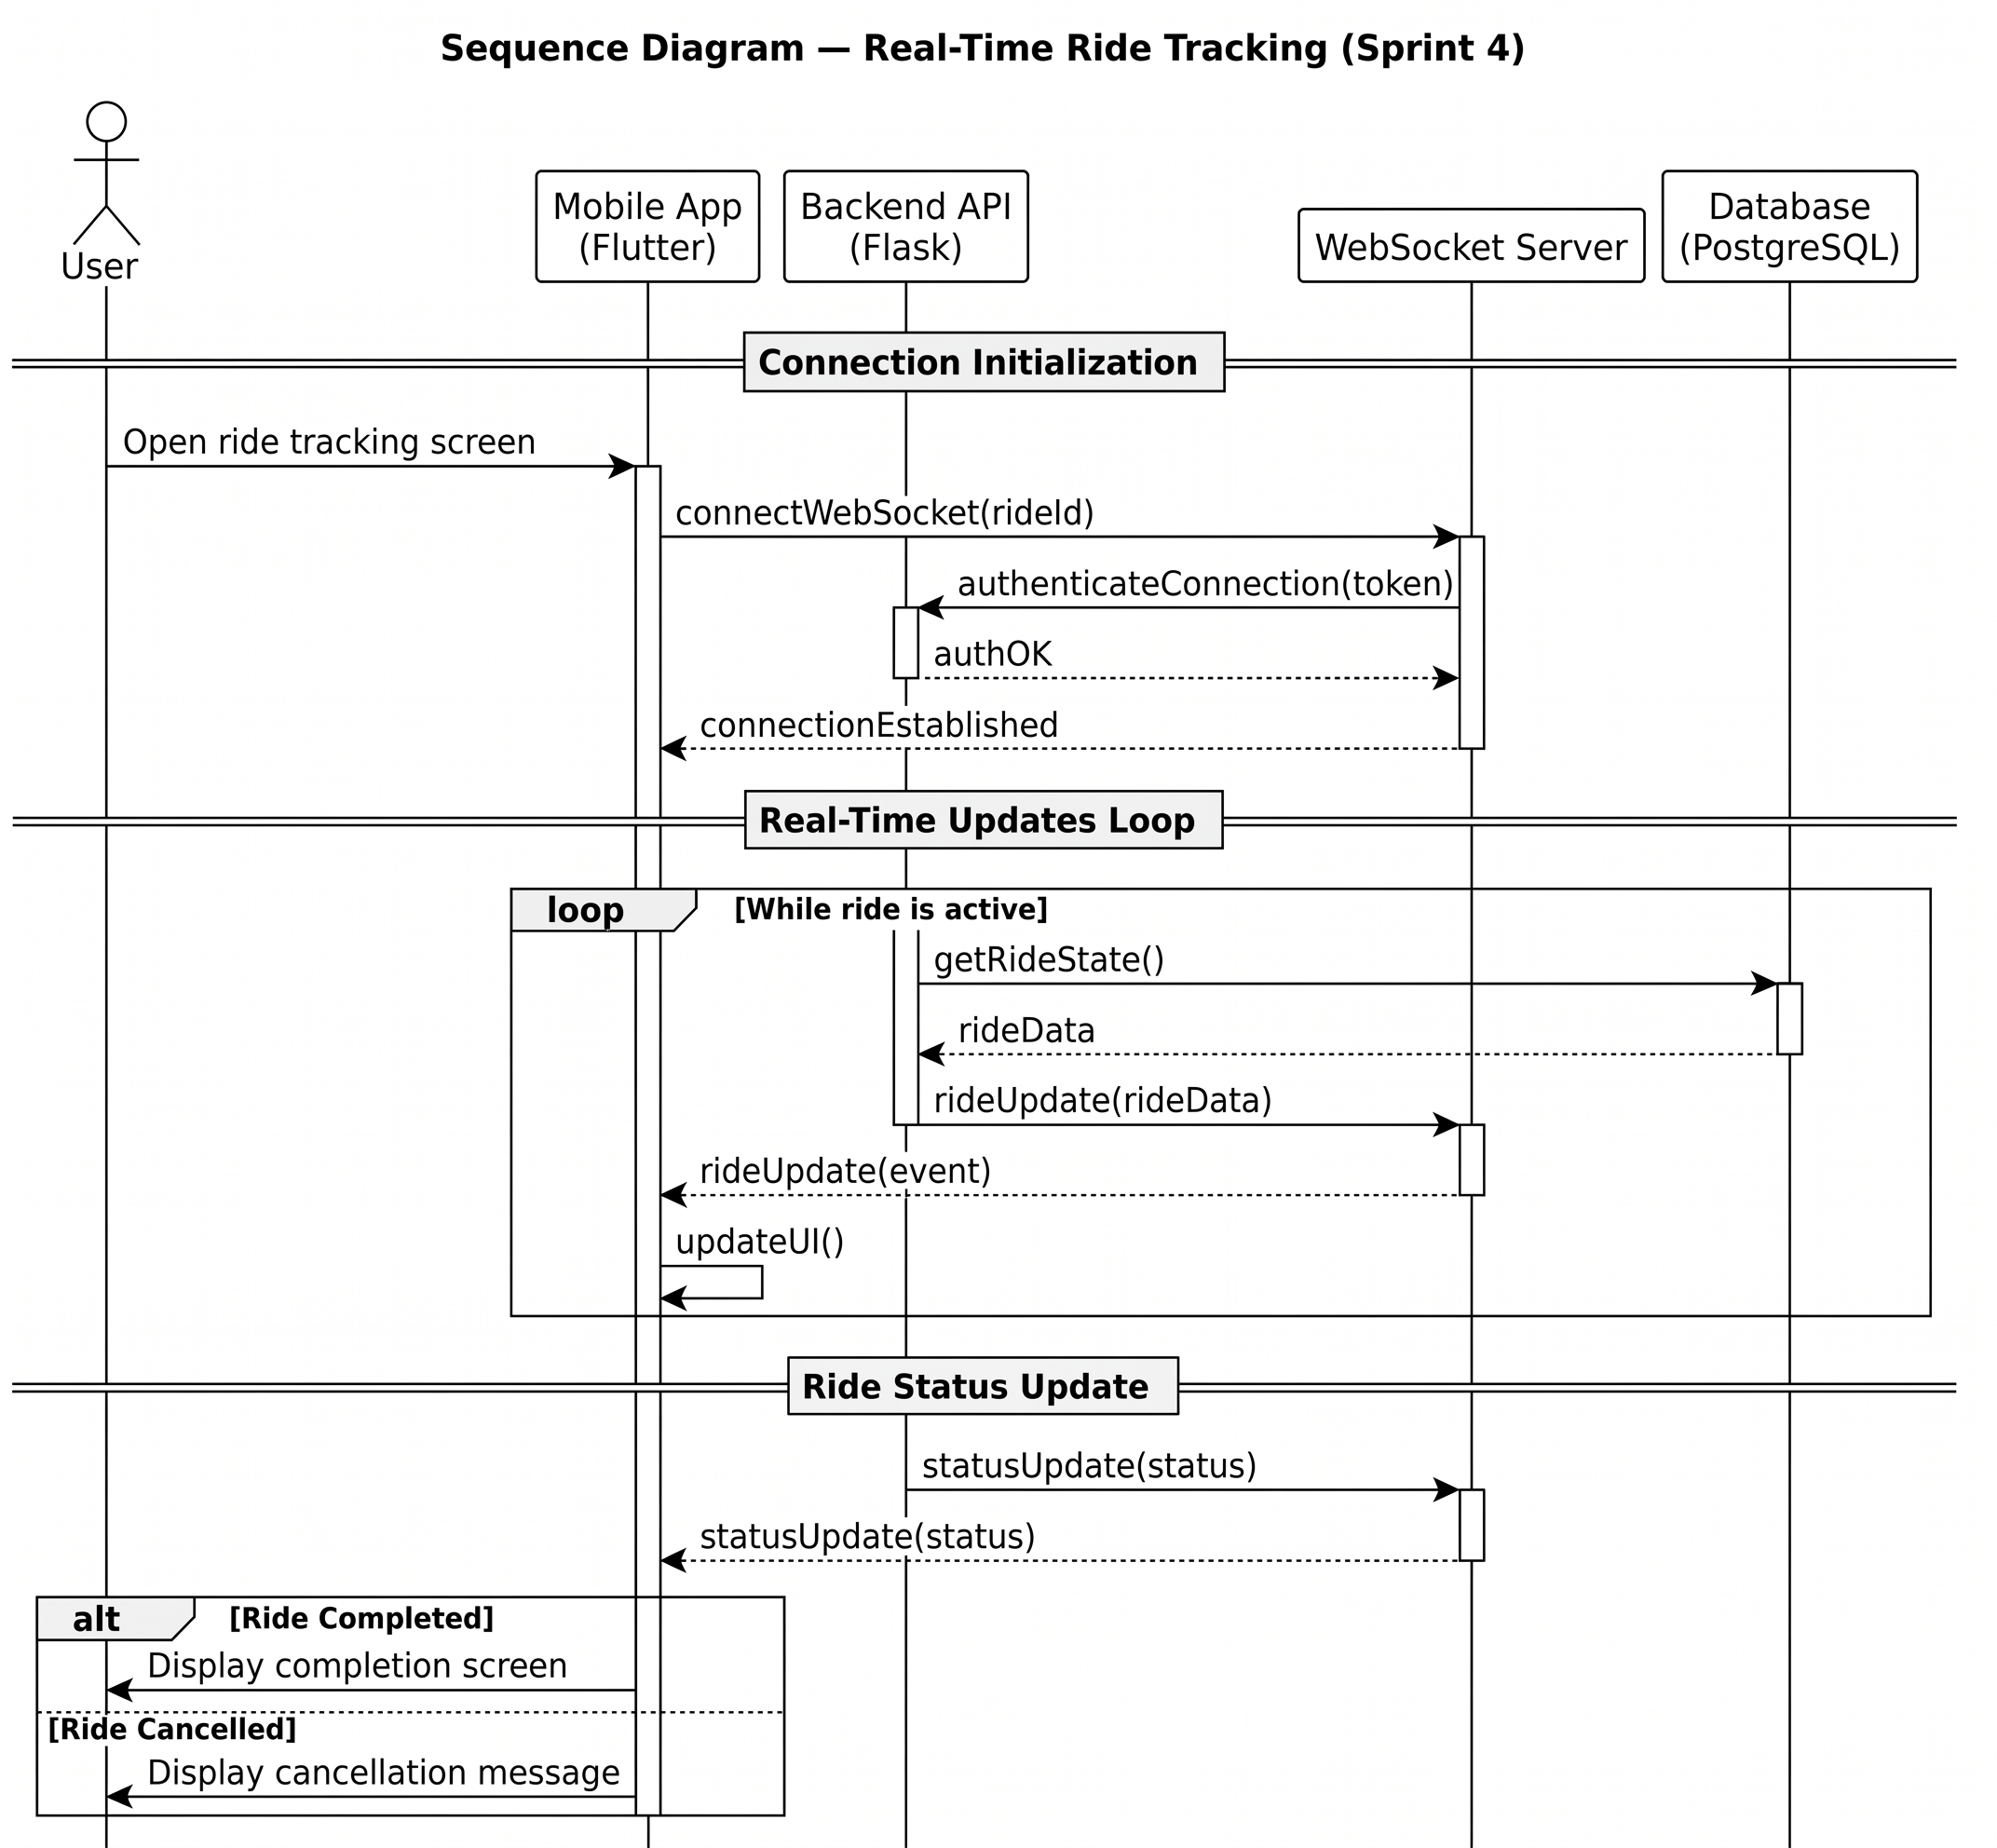
\includegraphics[width=0.9\textwidth]{images/diagrams/sequence_realtime.png}
\caption{Sequence Diagram — Real-Time Interaction}
\end{figure}

\subsection{Integration with Ride Lifecycle}

Real-time events are tightly coupled with the ride lifecycle.

For example:

\begin{itemize}
    \item When a ride status changes, an event is broadcast to all participants.
    \item When the driver updates their location, all passengers receive the new position.
\end{itemize}

This integration ensures that all users have a consistent and up-to-date view of the ride.

\subsection{TripCard Component}

To enhance user experience, a dynamic interface component called \textbf{TripCard} is displayed when an active ride is detected.

This component provides:

\begin{itemize}
    \item Real-time ride status
    \item Quick access to ride details
    \item Visual feedback on ride progression
\end{itemize}

The TripCard is updated dynamically based on real-time events received via WebSocket.

% \begin{figure}[H]
% \centering
% 
\includegraphics[width=0.4\textwidth]{images/chapter4/tripcard.png}
% \caption{TripCard Interface}
% \end{figure}

\subsection{User Interface Integration}

The real-time features are reflected in:

\begin{itemize}
    \item Live map updates
    \item Dynamic ride status display
    \item Interactive ride tracking interface
\end{itemize}

\subsection{Sprint Validation}

The following scenarios were tested:

\begin{itemize}
    \item Real-time reception of ride status updates
    \item Live driver location tracking
    \item System behavior under connection loss
    \item Fallback to periodic updates when needed
\end{itemize}

These tests ensured that the real-time system is robust and reliable.

% =========================================================
\section{Conclusion}

This chapter presented the implementation of the core ride management system and its extension with real-time interaction capabilities.

The integration of a structured ride lifecycle, strict business rules, and real-time synchronization ensures a consistent and responsive user experience.

The next chapter will focus on the intelligent components of the system, including the matching algorithm and machine learning-based prediction models.